\documentclass[tikz]{standalone}

\usepackage{tikz}
\usetikzlibrary{positioning, arrows.meta, shapes, snakes, shadings}
\usepackage{amsmath,amssymb,amsthm,pgfplots}

\pgfmathdeclarefunction{gauss}{2}{%
  \pgfmathparse{1/(#2*sqrt(2*pi))*exp(-((x-#1)^2)/(2*#2^2))}
}

% polychrome colour, kelly
\definecolor{kwhite}{RGB}{242,243,244}
\definecolor{kred}{RGB}{175,35,55}
\definecolor{kyellow}{RGB}{236,195,66}
\definecolor{kblue}{RGB}{41,103,160}
\definecolor{kolivegreen}{RGB}{47,60,40}
\definecolor{kyellowgreen}{RGB}{150,180,55}
\definecolor{kpurplishpink}{RGB}{218,147,171}
\definecolor{korange}{RGB}{229,137,50}
\definecolor{kpurple}{RGB}{128,89,143}
\definecolor{kreddishbrown}{RGB}{126,51,31}
\definecolor{kgreen}{RGB}{59,133,90}
\definecolor{kbuff}{RGB}{192,178,134}
\definecolor{klightblue}{RGB}{169,201,237}
\definecolor{kyellowishpink}{RGB}{236,151,127}
\definecolor{kgrey}{RGB}{132,132,130}
\definecolor{kyellowishbrown}{RGB}{96,70,40}
\definecolor{kreddishorange}{RGB}{210,96,52}
\definecolor{kpurplishred}{RGB}{166,76,107}
\definecolor{kgreenishyellow}{RGB}{219,210,69}
\definecolor{korangeyellow}{RGB}{235,168,59}
\definecolor{kviolet}{RGB}{93,80,146}
\definecolor{kblack}{RGB}{34,34,34}

\begin{document}
    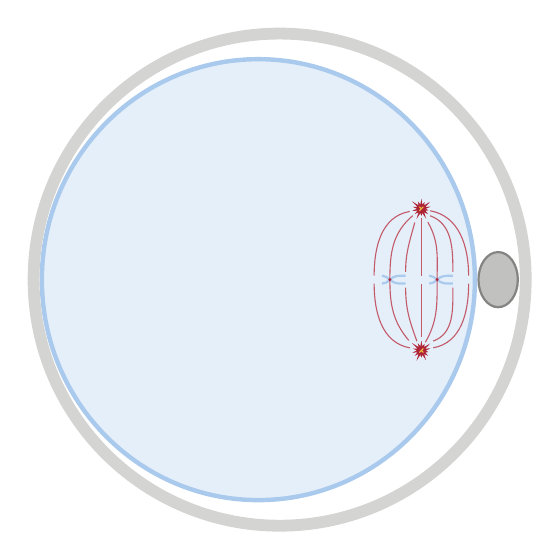
\begin{tikzpicture}
        % polar body 
        \draw[thick, kgrey, fill=kgrey!50] (5.775,3) circle[x radius=0.25, y radius = 0.35];
        
        % egg
        \draw[ultra thick, draw=klightblue, fill=klightblue!30] (2.73,3) circle[x radius=2.75, y radius=2.8];

        % chrom left
        \draw[thick, klightblue] (4.3,2.95) to[out=0, in=225] (4.4,3) to[out=45, in=180] (4.6,3.05);
        \draw[thick, klightblue] (4.3,3.05) to[out=0, in=145] (4.4,3) to[out=315, in=180] (4.6,2.95);
        
        % chrom right
        \draw[thick, klightblue] (4.9,2.95) to[out=0, in=225] (5,3) to[out=45, in=180] (5.2,3.05);
        \draw[thick, klightblue] (4.9,3.05) to[out=0, in=145] (5,3) to[out=315, in=180] (5.2,2.95);
        
        
        % top centrosome
        \node[name=tc1, shape=starburst, starburst points=14,
              starburst point height=1mm, inner sep=0.4mm,
              fill=kred] at (4.8,3.9) {};
        \draw[kyellow] (4.775,3.875) -- (4.825,3.925) (4.8,3.9) -- (4.775,3.925);
        \draw[thin, kred!75] (tc1.outer point 5) to[out=190, in=90] (4.2,3.05);
        \draw[thin, kred!75] (tc1.outer point 6) to[out=220, in=90] (4.4,3);
        \draw[thin, kred!75] (tc1.outer point 7) to[out=255, in=90] (4.6,3.1);
        \draw[thin, kred!75] (tc1.outer point 8) to (4.8,3.05);
        \draw[thin, kred!75] (tc1.outer point 9) to[out=300, in=90] (5,3);
        \draw[thin, kred!75] (tc1.outer point 10) to[out=340, in=90] (5.2,3.1);
        \draw[thin, kred!75] (tc1.outer point 11) to[out=350, in=90] (5.4,3.05);
        
        % bottom centrosome
        \node[name=tc2, shape=starburst, starburst points=14,
              starburst point height=1mm, inner sep=0.4mm,
              fill=kred] at (4.8,2.1) {};
        \draw[kyellow] (4.775,2.075) -- (4.825,2.125) (4.8,2.1) -- (4.825,2.075);
        \draw[thin, kred!75] (tc2.outer point 4) to[out=170, in=270] (4.2,2.95);
        \draw[thin, kred!75] (tc2.outer point 3) to[out=130, in=270] (4.4,3);
        \draw[thin, kred!75] (tc2.outer point 2) to[out=110, in=270] (4.6,2.9);
        \draw[thin, kred!75] (tc2.outer point 1) to (4.8,2.95);
        \draw[thin, kred!75] (tc2.outer point 14) to[out=60, in=270] (5,3);
        \draw[thin, kred!75] (tc2.outer point 13) to[out=20, in=270] (5.2,2.9);
        \draw[thin, kred!75] (tc2.outer point 12) to[out=10, in=270] (5.4,2.95);
        
        % two kinetochores
        \draw[draw=none, fill=kred] (4.4,3) circle[radius=0.02];
        \draw[draw=none, fill=kred] (5,3) circle[radius=0.02];

        \draw[draw=none, fill=kgrey!35, even odd rule]
            (3,3) circle[radius=3.2] (3,3) circle[radius=3.05];
%        \draw (3,3) circle[radius=3.2];
        
%        \draw[help lines, step=0.1] grid(6,6);
    \end{tikzpicture}   
\end{document}